\section{Feature Matching}
Feature: measured characteristic of (part of) a pattern / object\\
Goal: efficient matching


Features shoud overcome large variations in
\begin{enumerate}
	\item Viewpoint
	\item Illumination
	\item Background
	\item Occlusions
	\item Scale change
	\item Deformation
	\item Perspective Deformation
	\item Blur
\end{enumerate}

A feature should capture something \textbf{discriminative} about a well \textbf{localisable} patch of a surface

\subsection{Detector}

The detector typically yields image points. Corners are the most prominent example of so-called `Interest Points’, i.e. points that can be well localised in different views of a scene

\subsubsection{Uniqueness of a patch}
How do the patterns change upon a shift?\\
\textit{flat region}: no change in all directions\\
\textit{edge region}: no change along edge direction\\
\textit{corner} : significant change in all directions\\
\\
Compare each pixel before and after by summing up the squared differences (SSD) - this defines an error $E(u,v)$. Shift in x-direction: $u$, in y-direction:$y$.
$$ E(u,v) = \sum_{(x,y)\in W} [I(x+u, y+v) - I(x,y)]^2 $$
$$ E(u,v) = \sum_{(x,y)\in W} [u v] \underbrace{\begin{bmatrix}
I_x^2&I_xI_y\\
I_yI_x&I_y^2\\
\end{bmatrix}}_H \begin{bmatrix}
u\\
v\\
\end{bmatrix} $$
Want E(u,v) to be \textbf{large} for small shifts in \textbf{all} directions - the minimum is given by the smaller eigenvalue of H.

\subsubsection{The Harris corner detector}
$$ R = det(H) - k*trace(H)^2 $$
When $|R|$ is small, which happens when $\lambda_1$ and $\lambda_2$ are small, the region is flat.\\
When $R<0$, which happens when $\lambda_1$>>$\lambda_2$ or vice versa, the region is an edge.\\
When $|R|$ is large, which happens when $\lambda_1$ and $\lambda_2$ are large and $\lambda_1 ~\lambda_2$, the region is a corner.

\subsection{Descriptor}
Descriptors then are a vector of measurements taken around each such point


We need to describe their surrounding image patch such we can discriminate between them, i.e. we need to build a feature vector for the patch \&
Invariance under geom./phot. change

\subsubsection{Deformations under projections (geom. change)}
\begin{enumerate}
	\item similarity 4DOF
	\item affinity 6DOF
	\item projectivity 8DOF
\end{enumerate}

Complexity of the groups goes up with the generality of the viewing conditions, and so does the complexity of the group’s invariants. Fewer invariants are found going from top to bottom

\subsubsection{Photometric changes}
\begin{itemize}
	\item Contrasts (intensity differences) let the non-linear offsets cancel; hence gradients are good !
	\item Moreover the orientation of gradients in the color bands is invariant under their linear changes, as is the intensity gradient orientation in case the scale factors are identical; this is indeed relevant if the illumination changes its intensity, but not its color, which is typically assumed.
	\item But even under changing color of the illumination, in practice edge orientations tend to remain the same.
\end{itemize}

\subsection{Matching}
\begin{itemize}
	\item Interest points are matched on the basis of their descriptors
	\item E.g. nearest neighbour, based on some distance like Euclidean or Mahalanobis; good to compare against 2nd nearest neighbour: OK if difference is big; or fuzzy matching w. multiple neighbours
	\item Speed-ups by using lower-dim. descriptor space (PCA) or through some coarse-to-fine scheme (very fast schemes exist to date!)
	\item Matching of individual points typically followed by some consistency check, e.g. epipolar geometry, homograpy, or topological
\end{itemize}

\subsection{The Patch}
\subsubsection{MSER - Maximally stable extremal regions}
\begin{enumerate}
	\item Start with intensity extremum
	\item Then move intensity threshold away from its value and watch the super/sub-threshold region grow
	\item Take regions at thresholds where the growth is slowest (happens when region is bounded by strong edges)
\end{enumerate}

\subsubsection{SIFT - Scale-Invariant Feature Transform}
Is a carefully crafted interest point detector + descriptor, based on intensity gradients and invariants under similarities, not affine like so far.\\
\\
\textbf{Descriptor} is based on blob detection - at several scales - that is local extrema of the Laplacian-of-Gaussian (LoG)

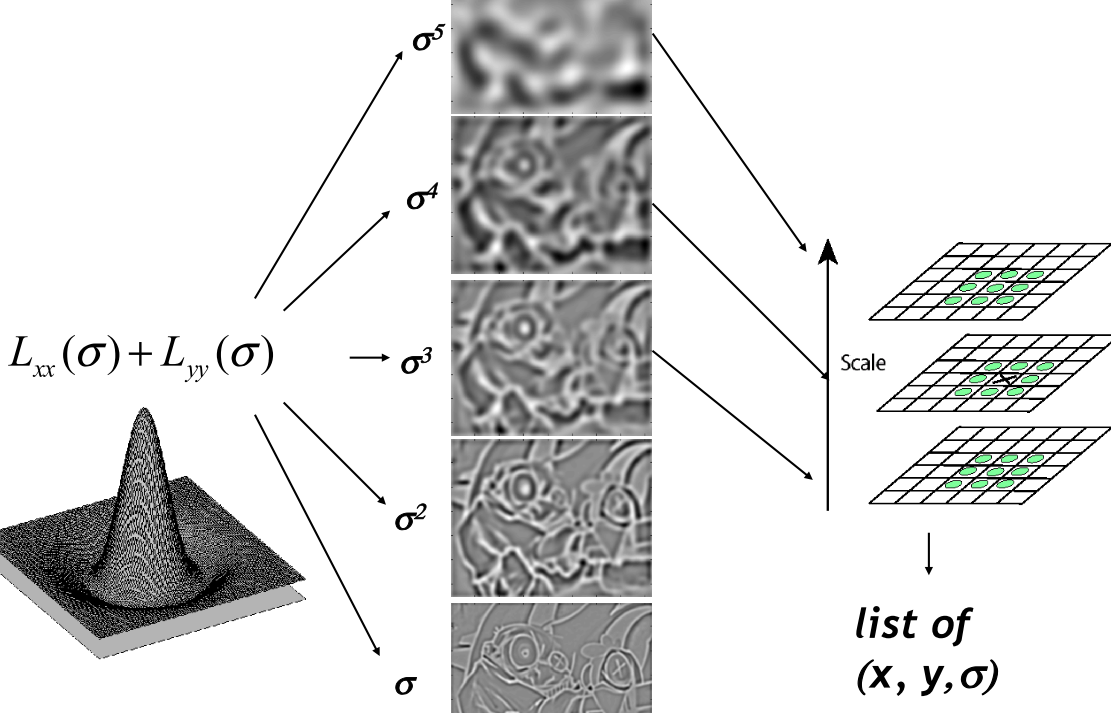
\includegraphics[width=0.7\columnwidth]{pictures/sift2}

\begin{itemize}
	\item Thresholded image gradients are sampled over a grid - Dominant orientation selection
	\begin{itemize}
		\item Compute image gradients of cell
		\item Build orientation histogram
		\item Find maximum of cell $\rightarrow$ orientation of cell
	\end{itemize}
	\item Create array of orientation histograms within blocks
	\item 8 orientations x 4x4 histogram array (! in picture only 2x2) = 128 dimensions
	\item Apply weighting with a Gaussian located at the center
	\item Normalized to unit vector
\end{itemize}

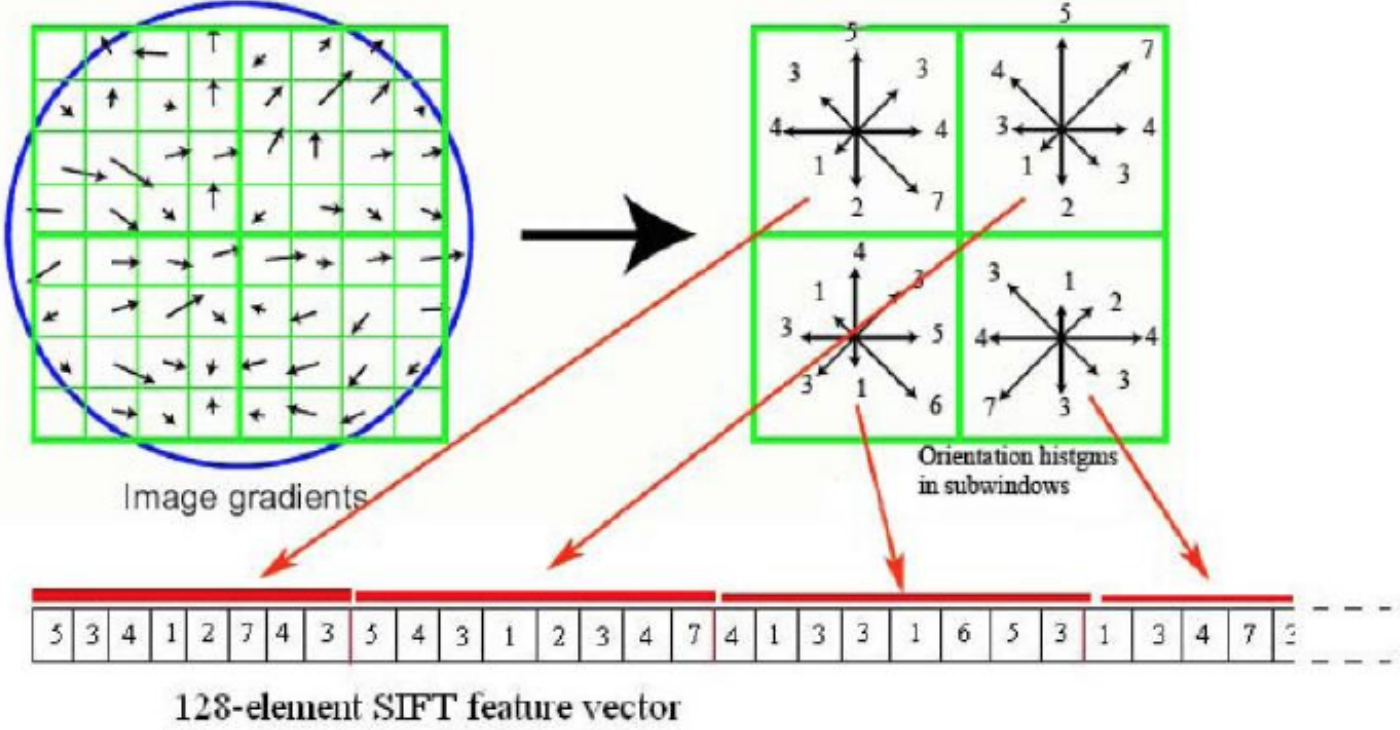
\includegraphics[width=\columnwidth]{pictures/sift}

\subsubsection{SURF - efficient alternative to SIFT}
no further infos